
\lecture{Examples of the Normal Distribution}{normal-distributions-examples}
\section{Examples of the Normal Distribution}

\title{Examples of the Normal Distribution}
\subtitle{Moar Normal!}

%\author{Kelly Black}
%\institute{Clarkson University}
\date{31 January 2014}

\begin{frame}
  \titlepage
\end{frame}

\begin{frame}
  \frametitle{Outline}
  \tableofcontents[hideothersubsections,sectionstyle=show/hide]
\end{frame}


\subsection{Clicker Quiz}


\iftoggle{clicker}{%
  \begin{frame}{Clicker Quiz}

    What is the probability that a random variable that follows a
    standard normal will be less than -0.45?

    \vfill

    \begin{tabular}{l@{\hspace{3em}}l@{\hspace{3em}}l}
      A:  .3264  & B: .3632  & C: .6736
    \end{tabular}

    \vfill
    \vfill
    \vfill

  \end{frame}
}


\subsection{Examples}

\begin{frame}
  \frametitle{Example}

  You are examining a portfolio of stocks. The total change in the
  value of an individual stock is normally distributed with a mean of
  0.5 and a standard deviation of 4.4. You want to decide which ones
  are in the top 25\% in gains based solely on the price change. What
  is the cut off?

  \vfill

  \only<2->{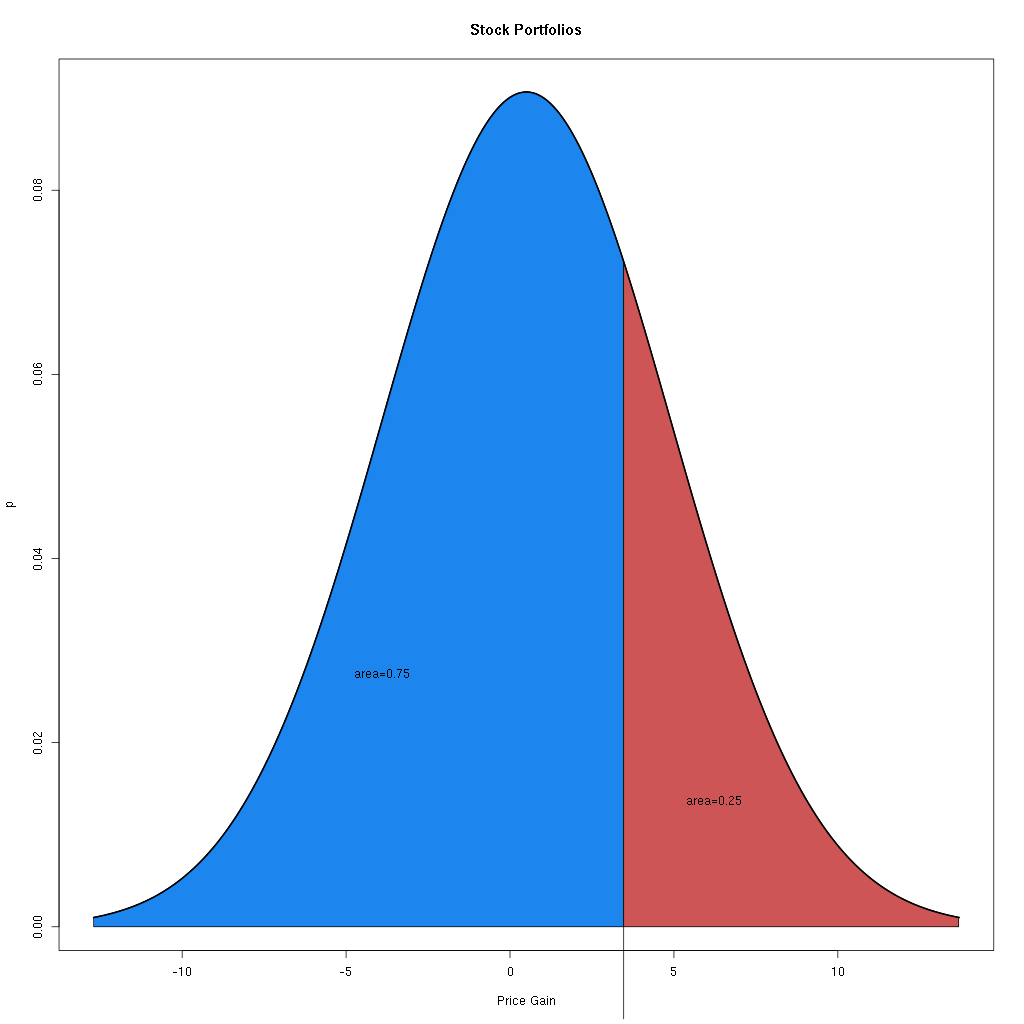
\includegraphics[width=12em]{img/topStockPicks}}

  \vfill


\end{frame}





\begin{frame}
  \frametitle{Example}

  A random variable has a mean of 3.0 and a standard deviation of
  4.5. If I take one sample what is the probability that it is less
  than zero?

  \vfill

  \only<2->{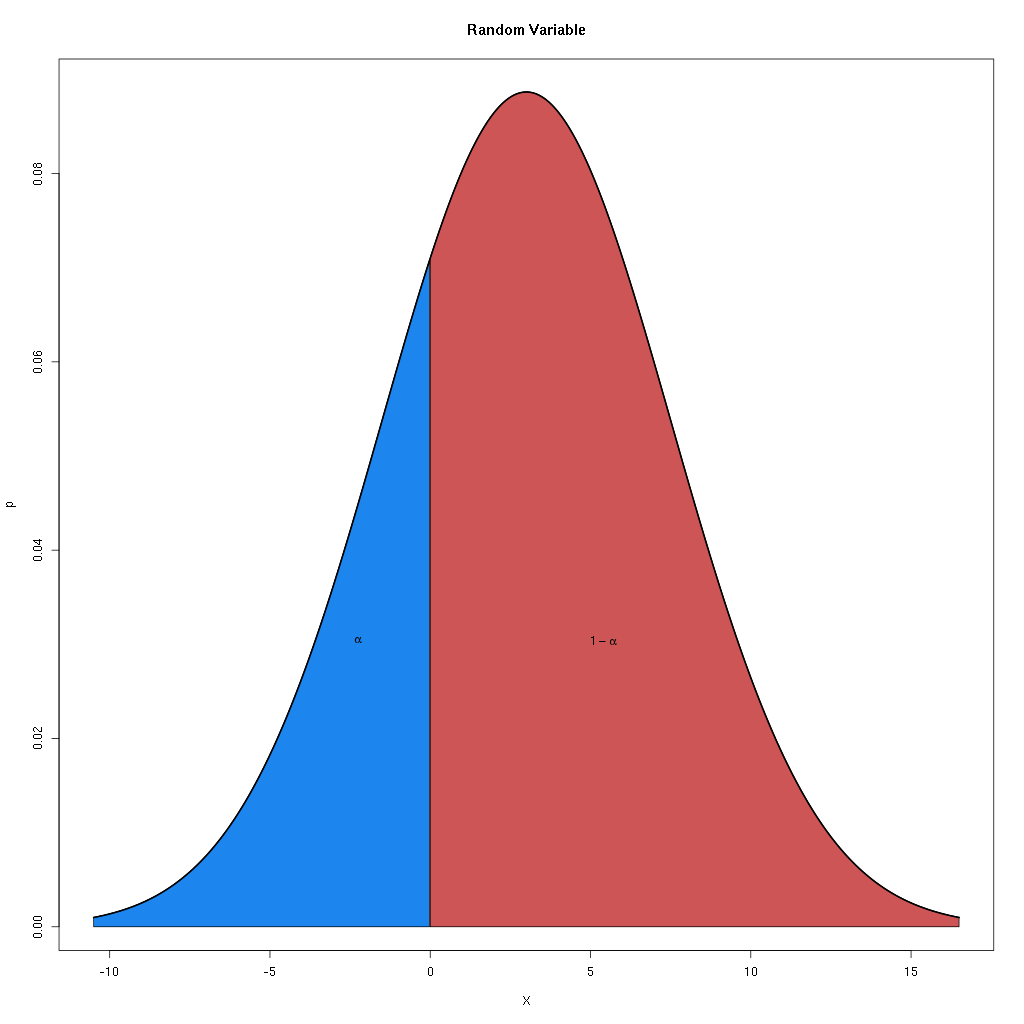
\includegraphics[width=12em]{img/normalRVMean3}}

  \vfill

%  \only<2->
%  {
%    If I take four samples what is the probability that it is less
%    than zero?
%  }
%
%  \vfill

\end{frame}

\iftoggle{clicker}{%
  \begin{frame}
    \frametitle{Clicker Quiz - Starting Salaries}

    The mean starting salaries for business majors is \$56,000 with a
    standard deviation of \$5,000. What is the probability that a
    randomly chosen business major will have an offer of more than
    \$63,000 per year?

    \vfill

    \begin{tabular}{l@{\hspace{3em}}l@{\hspace{3em}}l}
      A:  0.0808  & B: 0.919  & C: 1.4
    \end{tabular}

    \vfill
    \vfill
    \vfill



  \end{frame}
}





\iftoggle{clicker}{%
  \begin{frame}
    \frametitle{Clicker Quiz}

    The total change in a stock's price on one particular day has a
    mean of -.35\$ with a standard deviation of .86\$.  What is the
    probability that the price change in a randomly chosen stock will
    be more than zero?

    \vfill

    \begin{tabular}{l@{\hspace{3em}}l@{\hspace{3em}}l@{\hspace{3em}}l}
      A: 0.0516  & B: 0.3420 & C: 0.6580 & D: 0.9484
    \end{tabular}

    \vfill
    \vfill
    \vfill

  \end{frame}
}


\begin{frame}
  \frametitle{Example}

  A random variable has a mean of 12.0, and the probability that it is
  less than 8.0 is approximately 0.25. What is the standard deviation?

  \vfill

\end{frame}


\begin{frame}
  \frametitle{Example}

  A random variable has a mean of -2.0 and a standard deviation of
  5.0. Find the value, $x$, so that there is a probability of 0.30 that the
  random variable is bigger than than $x$.

  \vfill

\end{frame}




% LocalWords:  Clarkson pausesection hideallsubsections hideothersubsections
% LocalWords:  sectionstyle
